%%%%%%%%%%%%%%%%
%\chapter{Language Restrictions (Main Result: Theorems)}
%%%%%%%%%%%%%%%%

%State clearly definitions, assumptions, and proofs. The document will be archived for posterity and your name will be associated with any mistakes you make.

%%%%%%%%%%%%%%%%%%%%%%%%%%%%%%%%
\chapter{Design}
%%%%%%%%%%%%%%%%%%%%%%%%%%%%%%%%
% Introduce and discuss the design decisions that you made during this project.
% Highlight why individual decisions are important and/or necessary. Discuss
% how the design fits together.
% Use as much as needed.

The goal is to port Java to native restrictions with a minimal set of changes to the JDK. We want Java to behave exactly like Native Image, and crash for the exact same reasons that Native Image does. Our design focuses on labsjdk-21, which is a mirror of openjdk-21. 
This section explains how semantic changes can be modeled through the concept of (1) native restrictions, (2) how defining scopes in the JDK enables us to express these changes, and (3) how we improve Native Image usability.

%%%%%%%%%%%%%%%%%%%%%%%%%%%%%%%%
\section{Native Restrictions}
%%%%%%%%%%%%%%%%%%%%%%%%%%%%%%%%
We introduce the concept of native restrictions to represent the set of semantics that Java is running with. These restrictions modify the way dynamic class loading, reflection and the \verb|SecurityManager| behave at runtime. Each feature can be individually selected to run under native restrictions, and behave like in Native Image, or not, in which case it behaves like Java.
At the two end of the spectrum of the native restrictions, we have that (1) when no restrictions are applied, Java behaves according to the Java Language Specification, (2) and when all the restrictions are applied, Java behaves according to the Native Image Semantics, as presented in Section~\ref{native_image_specs}. 

The restriction mode for Java can be set using the System property \verb|language.restriction|. At runtime, we perform checks for an expected behaviour depending on whether the feature is running under native restrictions or not, thus effectively changing the semantic of Java.
% Moreover, proving that Java can behave like Native Image enables us to drive the specification of Native Image.

%%%%%%%%%%%%%%%%%%%%%%%%%%%%%%%%
\section{Native Restrictions Scopes and Checks}
%%%%%%%%%%%%%%%%%%%%%%%%%%%%%%%%
The challenge in designing the semantics changes is that they require us to differentiate runtime from build time behavior, but also JDK calls from user calls.

One possible approach relies on bytecode transformation, but these transformations are both complex to implement and introduce non-trivial changes to the compiler. 
Instead, we use the notion of scopes to open regions of codes where the JDK is not constrained to native restrictions.
The JDK bypasses the native restrictions checks either because it attempts to define an internal class at runtime or for performance reasons.
% These scopes enable us to differentiate JDK calls from user calls at runtime.
% This regions are explicitly delimited such that only code for the JVM is executed, arbitrary user-code remains restricted.

More formally, let \verb|C| and \verb|A| be two classes or interfaces (for the rest of the thesis the term class will refer to both classes and interfaces), let \verb|c| be a method of \verb|C|, and assume the existence of a mechanism to open scopes. As shown in Figure~\ref{fig:scopes}, \verb|c| opens a scope S, invokes the method \verb|a| of \verb|A|, and closes S when it returns from \verb|a|.
The method \verb|a| invokes a method \verb|b| that performs some checks.
Then if \verb|c| is invoked, the restrictions checks in \verb|b| will be ignored, as they are included in S.
If \verb|a| is invoked by another caller than \verb|C.c|, the checks in \verb|b| will be performed.

\begin{figure}[ht]
    \centering
\begin{lstlisting}[language=Java]
class A {
    public static void a() {
        b(); 
    }
    public static void b() {
        // native restrictions check
    }
} 
class C {
    static void c() {
       ...
       // start of scope S
       A.a();
       // end of scope S
       ...
    }
}
\end{lstlisting}
    \caption{Using scopes}
    \label{fig:scopes}
\end{figure}

Native restrictions checks refer to runtime checks that we use to enforce native restrictions. They usually consists in a first check to see if a scope is open and if the concerned feature is not running under native restrictions, in which case the check returns without side effect. Additional operations can be conducted, such as checking if an element is registered for reflection. 

In the following subsections we show in more details how these scopes were chosen for each feature and that they are correct according to Native Image semantics.

%%%%%%%%%%%%%%%%%%%%%%%%%%%%%%%%
\subsection{Dynamic Class Loading}
%%%%%%%%%%%%%%%%%%%%%%%%%%%%%%%%
As mentioned in the background section, Native Image does not generally support dynamic class loading unless the class is preloaded, that the class is linked at build time and registered for reflection.
To simulate this behaviour, we require, under native restrictions, that loading a class at runtime with \verb|java.lang.ClassLoader#defineClass1|, \verb|java.lang.ClassLoader#defineClass2| or \verb|java.lang.ClassLoader#defineClass0| results in a \verb|UnsupportedOperationException|, unless the class is registered for reflection and is on the classpath.

The method \verb|java.lang.ClassLoader#loadClass| can be called from the JVM to initiate class loading, or directly from user-code. In the former case we do not want an exception to be thrown, in the latter, we want to throw an exception to prevent user from defining an arbitrary class at runtime.
To differentiate these paths, we introduce the wrapper method \verb|java.lang.ClassLoader#runtimeLoadClass|. Instead of directly calling \verb|loadClass|, the JVM now invokes the wrapper function, which dispatches the call to the delegate class loader, as intended when running without restrictions. As shown in Figure~\ref{fig:load_class}, the JVM is the only entry point.
Invoking \verb|runtimeLoadClass| opens a scope, which closes on \verb|defineClass1|'s return.
Directly calling \verb|loadClass| does not open the scope and \verb|defineClass1| will throw an \verb|UnsupportedOperationException|.
To simulate class preloading, we modify \verb|java.lang.ClassLoader#findLoadedClass|.
Under native restrictions, we check if the scope is open, in which case \verb|findLoadedClass| simply returns. If the scope is not open and the class is not registered a \verb|MissingReflectionRegistrationError| is thrown.
If the class is registered, then we simulate the class being preloaded by invoking \verb|Class#forName| with the application class loader to load the class. Attempting to load a class that is not on the classpath will still result in an \verb|UnsupportedOperationException|.

% Before \verb|loadClass| invokes \verb|defineClass1|, it first calls \verb|java.lang.ClassLoader#findLoadedClass|. This method can immediately returns the class if it was already resolved before, in which case \verb|loadClass| does not invoke \verb|defineClass1|.
% Under native restrictions, we check if the scope is open, in which case \verb|findLoadedClass| simply returns. If the scope is not open and the class is not registered a \verb|MissingReflectionRegistrationError| is thrown.
% If the class is registered, then we simulate the class being linked at build time by invoking \verb|Class#forName| with the application class loader to load the class. Attempting to load a class that is not on the classpath will still result in an \verb|UnsupportedOperationException|

% If not preloaded, then a class may be defined at runtime only if resolving the class or interface was required by one of the following instructions:
% anewarray, checkcast, getfield, getstatic, instanceof, invokedynamic, invokeinterface, invokespecial,
% invokestatic, invokevirtual, ldc, ldc\_w, multianewarray, new, putfield, and putstatic.

\begin{figure}
    \centering
    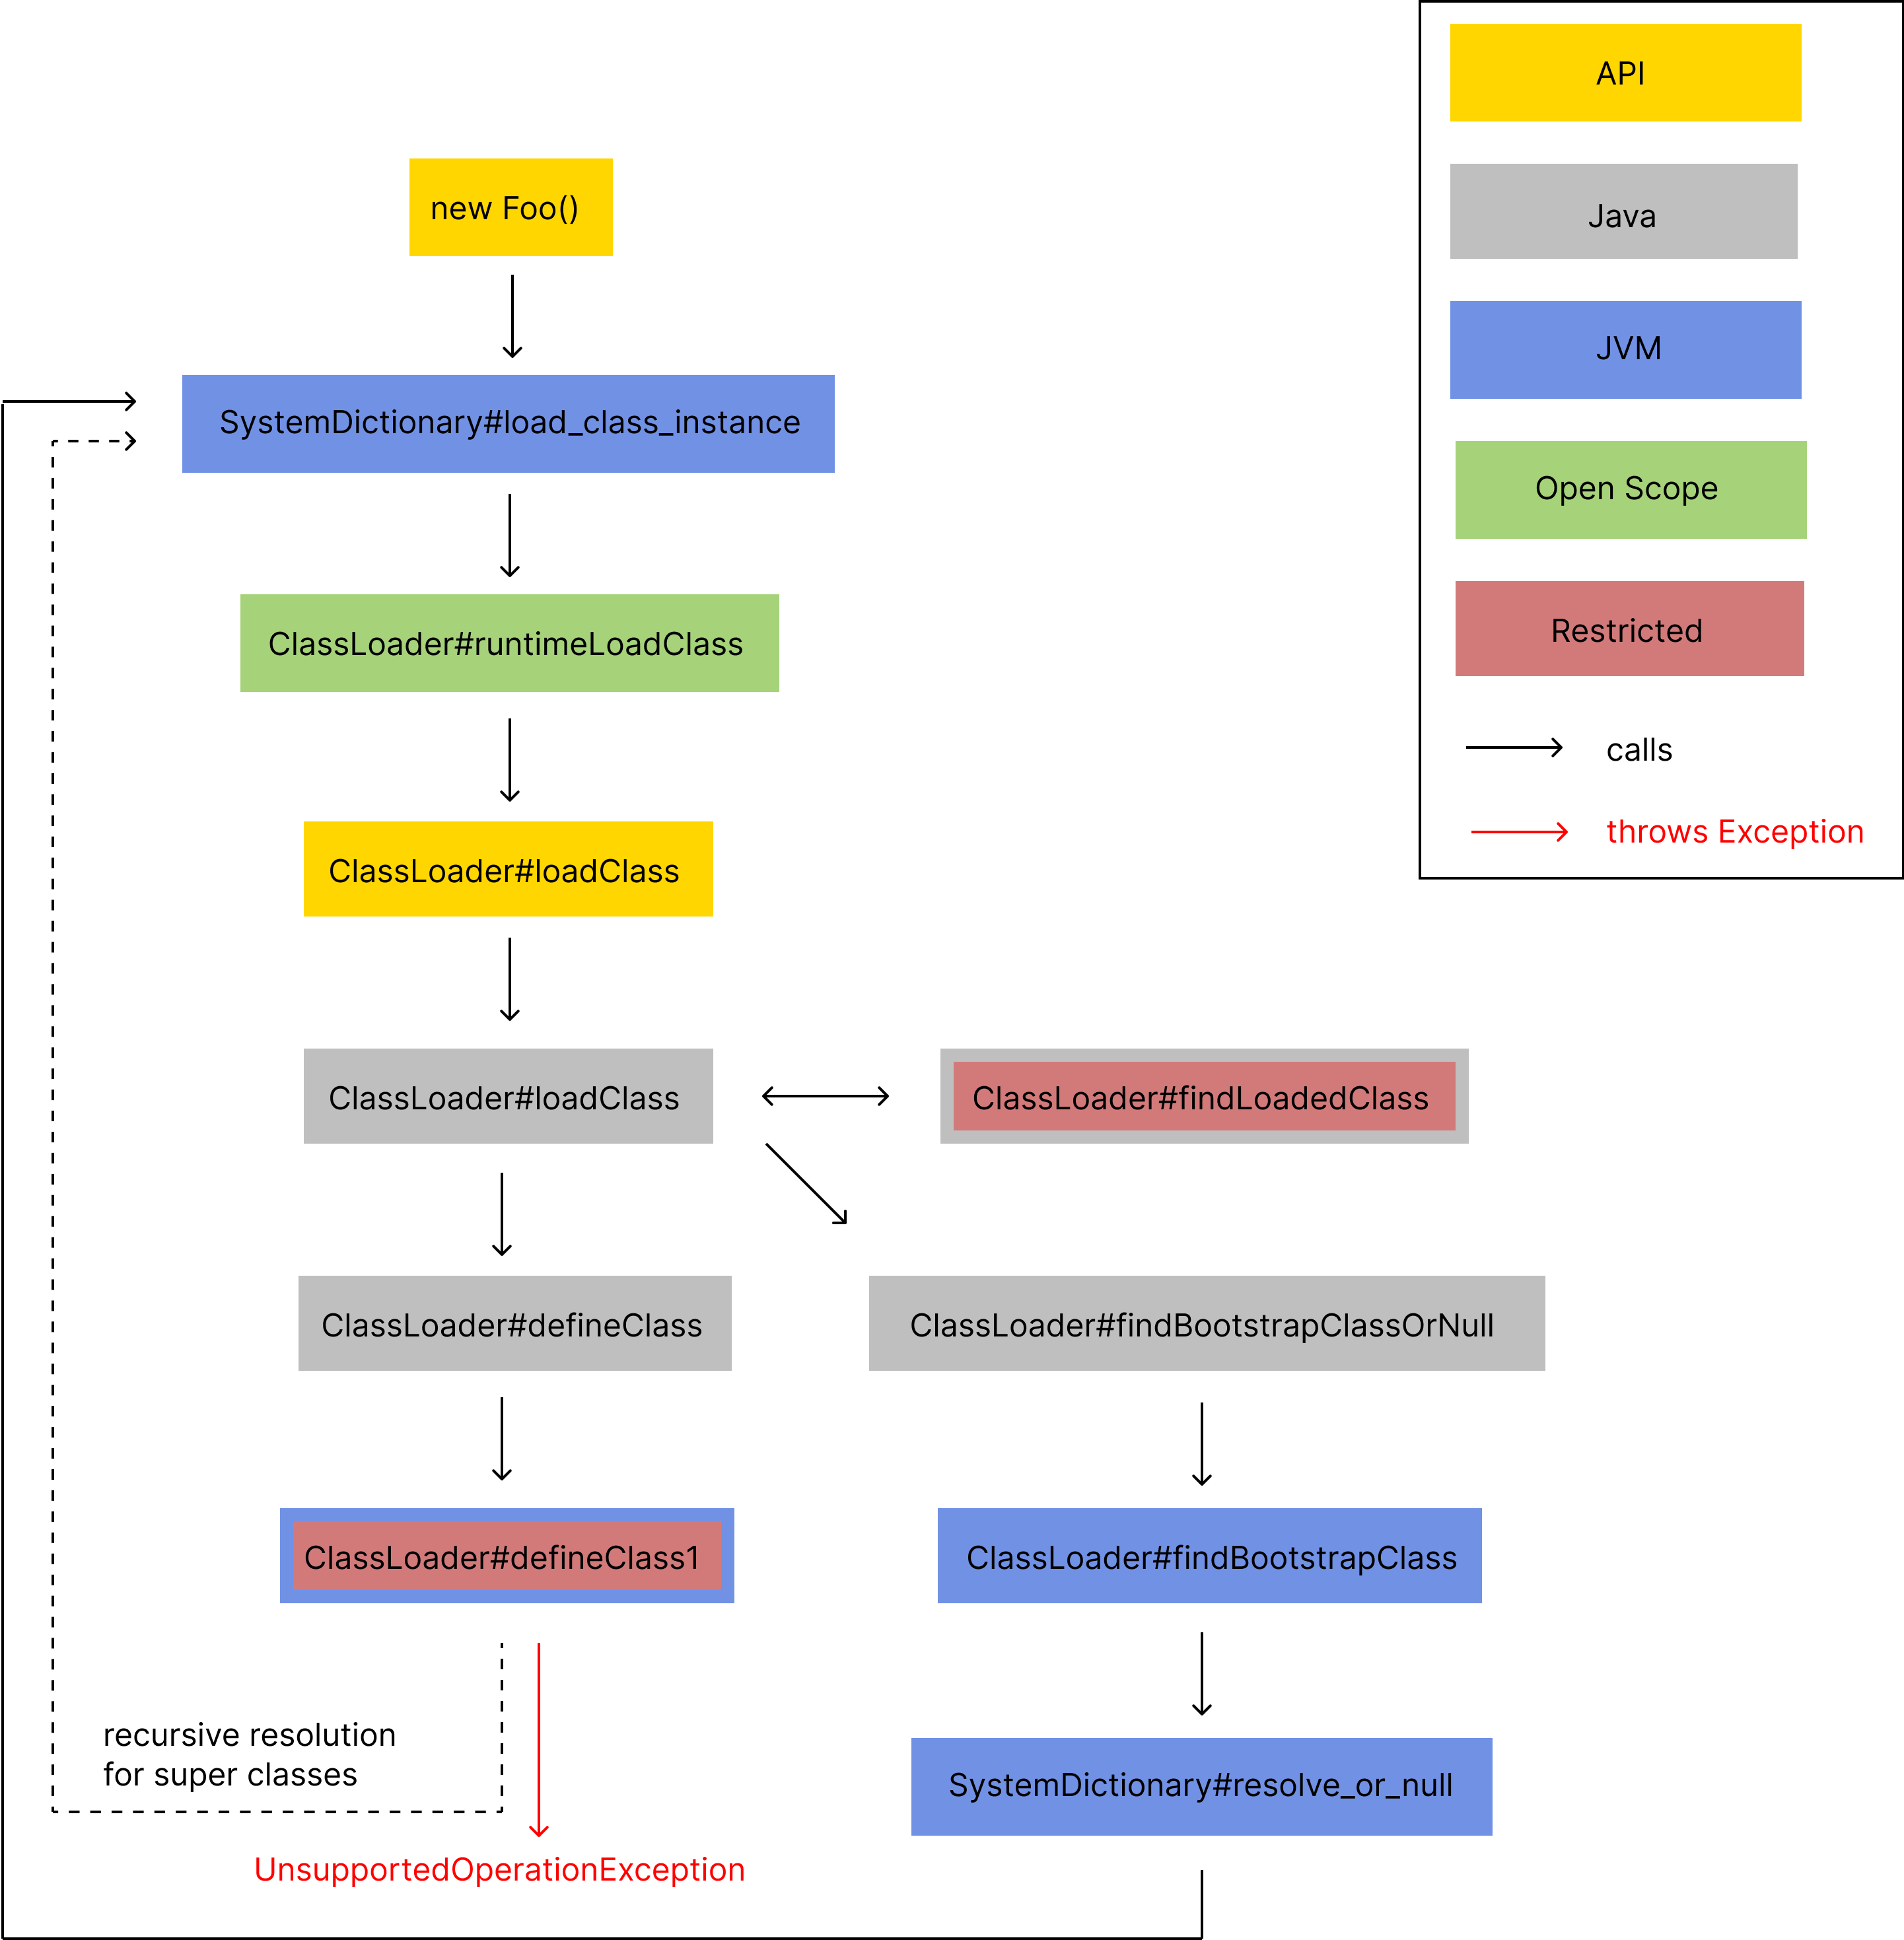
\includegraphics[scale=0.5]{resources/Group 403.png}
    \caption{Calling sequence for class loading, with the wrapper function \texttt{runtimeLoadClass} and scopes to support dynamic class loading at runtime.}
    \label{fig:load_class}
\end{figure}

Dynamic invocation required multiple design iterations to keep the changes to a minimum. Figure~\ref{fig:define_class_0} shows all the entry points from which \verb|java.lang.ClassLoader#defineClass0| can be invoked to define a hidden class, and illustrates the final state of the design.  
Under native restrictions the methods \verb|metafactory| and \verb|altMetafactory| of \verb|java.lang.invoke.LambdaMetfactory| cannot be invoked directly form user code as this would allow for the execution of arbitrary code at runtime, unless the invocation is part of the \verb|invokedynamic| instruction. To differentiate both paths, we open a scope in \verb|java.lang.BootstrapMethodInvoker#invoke|, which is invoked by the JVM in the process of linking the \verb|CallSite| to resolve (and invoke) the bootstrap method, if and only if Native Image also compiles this bootstrap method at build time
Figure~\ref{fig:define_class_0}, shows that moving the opening of the scope up or down on the stack trace would mean introducing an additional change because of the branching out. We also do not have the required metadata on the bootstrap method to place it in the JVM.   

% In the first implementation, scopes where open in \verb|java.lang.invoke.LambdaMetfactory| in both the \verb|metafactory| and the \verb|altMetafactory| methods, if the invocation was part of the \verb|invokedynamic| instruction.
% This initial design had two issues. The first one being that it required us to check the stack trace and see if the \verb|java.lang.invoke.BootstrapMethodInvoker| was on the path to differentiate JVM from user calls. The second was that it was too restrictive, thus incorrect according to Native Image semantic, as the only bootstrap method that where allowed to be resolved at runtime where for lambda expressions.
% Instead, we placed the scope lower on the stack trace, in the \verb|java.lang.BootstrapMethodInvoker#invoke| method. This method is invoked by the JVM in the process of linking the \verb|CallSite| to resolve (and invoke) the bootstrap method. The scope is open only for bootstrap methods that Native Image compiles at build time.
% Figure~\ref{fig:define_class_0}, shows that moving the opening of the scope up or down on the stack trace would mean introducing an additional change because of the branching out. We also do not have the required metadata on the bootstrap method to place it in the JVM.   

Three main categories of user calls can result in the resolution of a method handle such that the JVM emits calls to define internal classes of the JDK at runtime: (1) the invocation, and (2) binding of a method handle and (3) the lookup of an executable or field. As an optimization, the JVM compiles \verb|LambdaForm|, \verb|InjectedInvoker|, specialized \verb|BoundMethodHandle| and other automatically generated internal classes. 
In Native Image, these classes are either forced interpreted, or does not generate specialized code and letting Java under native restrictions define these classes does not contradict these semantics. As such, for performance reason, we opt to open scopes in the concerned methods, and let the JVM define these classes at runtime.

\begin{figure}
    \centering
    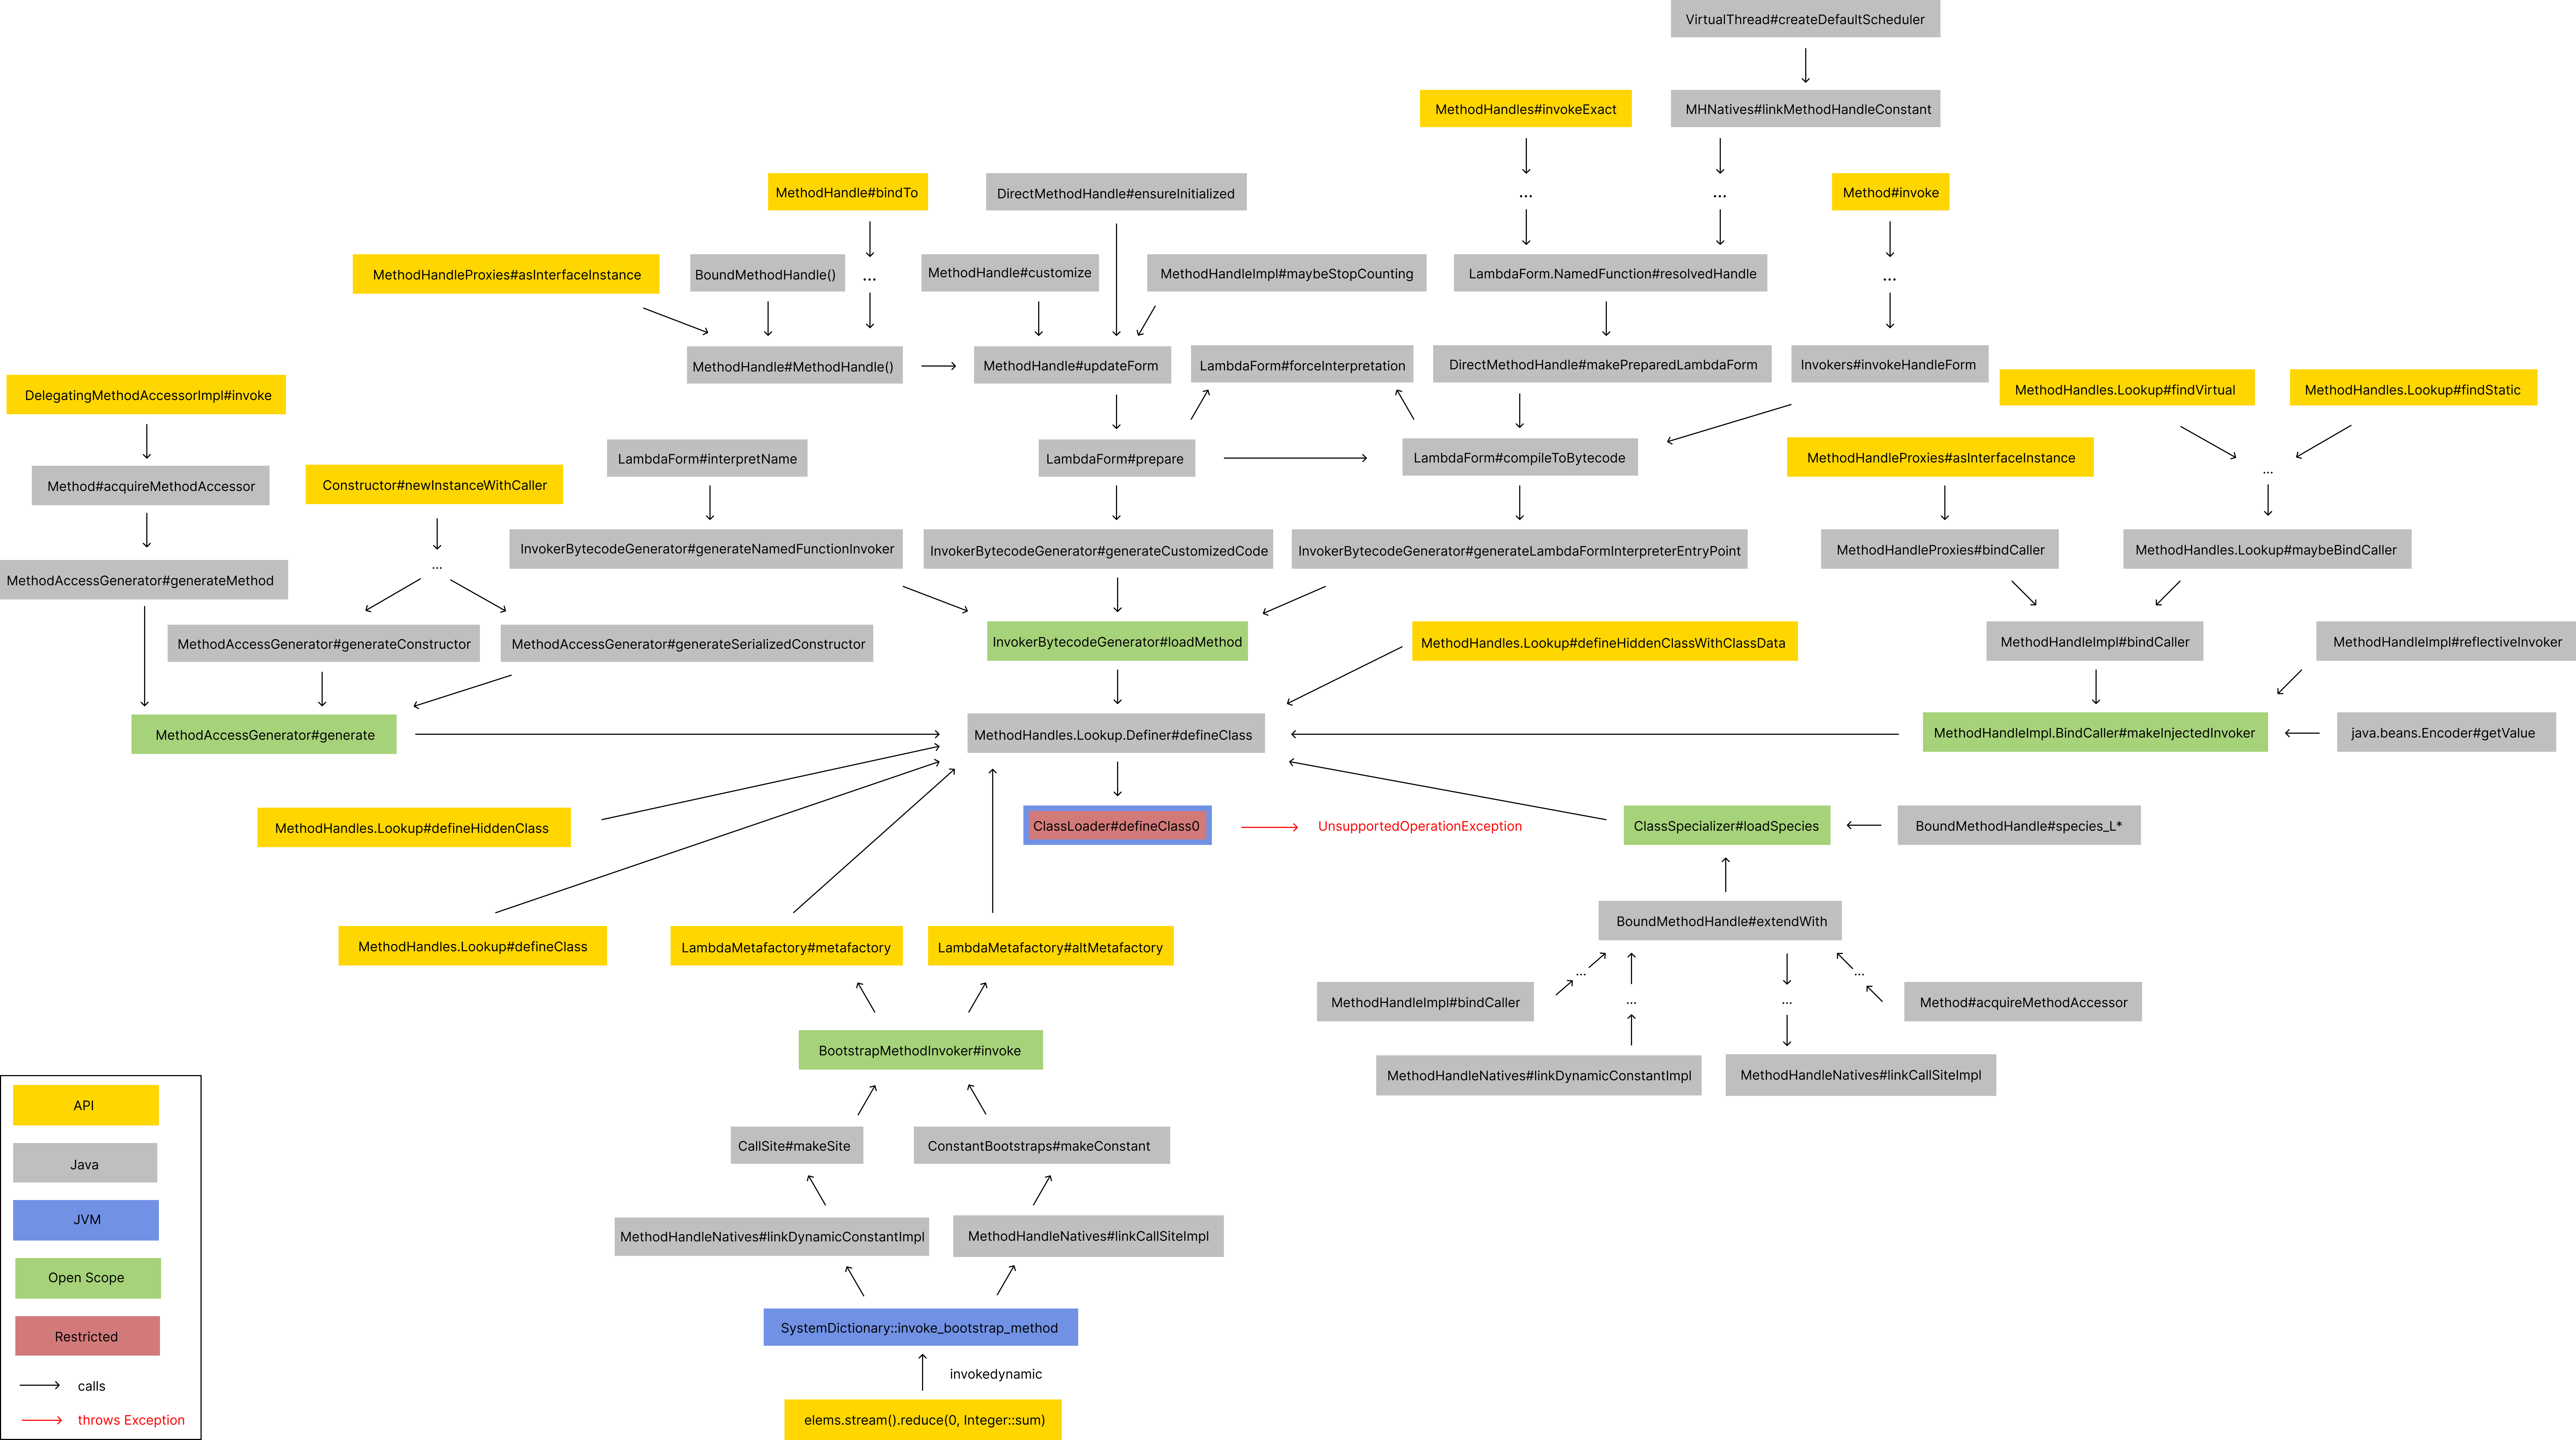
\includegraphics[angle=90,origin=c,scale=0.26]{resources/Group 401.png}
    \caption{Entry points for the method \texttt{java.lang.ClassLoader\#defineClass0}. For readability, the stack trace is not exhaustive and focuses on methods that have multiple callers.}
    \label{fig:define_class_0}
\end{figure}

% forgot to mention proxies and resource bundles

Finally, \verb|defineClass1|, \verb|defineClass2| and \verb|defineClass0| are all native methods. Since the Java Native Interface~(JNI)~\cite{noauthor_jni_nodate} enables downcalls to the JVM's implementation of the define class method, we insert the native restrictions checks in the \verb|SystemDictionary::resolve_from_stream| which is part of the common code for \verb|JVM_DefineClass| and \verb|JVM_DefineClassWithSource|. If none of the scopes are open, the call will result in an \verb|UnsupportedOperationException|. 

%%%%%%%%%%%%%%%%%%%%%%%%%%%%%%%%
\subsection{Reflection}
%%%%%%%%%%%%%%%%%%%%%%%%%%%%%%%%
Designing Java under native restrictions for reflection consists in adding native restrictions checks to all methods in the \verb|java.lang.Class| class, the package \verb|java.lang.invoke.reflect|, and \verb|jdk.internal.sun.misc.Unsafe| that returns a reflectively-accessed element (see Section~\ref{native_image_specs} for a detailed list of the checks). 
If the reflectively-accessed element is not registered for reflection, a \verb|MissingReflectionRegistrationError| is thrown.
To check if an element is registered, we load all reflection configuration files that are on the classpath and user defined. The actual code to parse the JSON configuration file and the data structure that holds the configuration are taken directly from Native Image, and offers an interface such that changes in Native Image code will not affect the Java mode.

Method handle resolution can occur, from the user perspective as a result of two operations. A first way is to dynamically invoke a method, the other way is via a lookup.
Similarly to reflection, \verb|java.lang.MethodHandles.Lookup| provides an API to look up \verb|Executables|, \verb|Fields|, and \verb|VarHandles|, and returns a method handle to access the element. Internally the method handle contains a \verb|MemberName| that encapsulate the element's declaring class, name, and its type parameters if it has any. 
In Native Image the \verb|MemberName| is resolved through reflection if the associated method handle is not intrinsic. In Java under native restrictions we introduce a reflective access check in the \verb|java.lang.invoke.MemberName#resolve|. 
For intrinsic method handles, we keep a hard-coded list of \verb|MemberName| that do not require reflection to be resolved. Scopes cannot be used in this situation, as invoking a method relies on these same intrinsic method handles.
Moreover, as parts of the internal code for the tracing agent uses lambda expressions to store the metadata, we also open a scope in \verb|MethodHandles#linkMethodHandleConstant| to prevent a loop.

% REST TO BE DETERMNINED....

%%%%%%%%%%%%%%%%%%%%%%%%%%%%%%%%
\section{Improving Usability}
%%%%%%%%%%%%%%%%%%%%%%%%%%%%%%%%
In this section, we will see how the Java mode fit in the overall Native Image usability plan by improving the turnaround for computing reachability metadata, facilitating debugging of user code and defining the expected behaviour of Native Image. 

%%%%%%%%%%%%%%%%%%%%%%%%%%%%%%%%
\subsection{Improving turnaround computation of reachability metadata}
%%%%%%%%%%%%%%%%%%%%%%%%%%%%%%%%
One of the main goal of this thesis is to streamline reachability metadata computation for users.
The first step in the computation of these metadata is the collection. To achieve this Native Image offers a tracing agent that automatically collect the reachability metadata required for an application. This agent omits to log metadata for certain JDK internal classes (the \verb|MethodHandle| and its subtypes, classes from the \verb|java.lang| package, etc.), because Native Image does not require these elements to be registered, as the reachability of these elements can be proven in the code.  

To simplify the work flow and provide more transparency, we implement a tracing agent in the Java mode. In essence, the tracing agent is simply another language restriction added to the JDK. It is designed to follow the exact same path during an execution as Java under native restrictions. Instead of performing restriction checks, the agent logs the reflectively-accessed elements and outputs a configuration at the end of the execution run.
This also offers the advantage of giving a concrete list of JDK internal classes and methods that are proven in the code.

Debugging is not an easy task. While it is possible to attach a java debugger to the image build process, debugging the image itself is trickier. 
%% TODO

We propose a new and optimized workflow for computing metadata: (1) run the agent, (2) test the configuration with Java under native restrictions, (3.a) if the execution did not result in an exception build the \textit{native-image}, (3.b) otherwise debug the application by attaching a Java debugger.

%%%%%%%%%%%%%%%%%%%%%%%%%%%%%%%%
% \subsection{Say Goodbye to GDB}
%%%%%%%%%%%%%%%%%%%%%%%%%%%%%%%%
% Debugging is not an easy task. While it is possible to attach a java debugger to the image build process, debugging the image itself is trickier.

% -----------------------------------
% Debugging a compiler is not as straightforward as debugging most other types of projects. There
% are two different parts. The first easier one is debugging the image construction. As it is written in
% Java, it is possible to attach a Java debugger on the code and debug it as most other programs. The
% error messages are understandable and usually allow to quickly find the issue. The second one,
% consisting in debugging the image, is harder. While most error messages can still help identifying
% the cause of the failures, a lot of them end in a segmentation fault, meaning the best ally for
% debugging images is GDB and the assembly code obtained using objdump. Sadly, a lot of useful
% tools, such as valgrind, are not implemented for RISC-V yet. Since the backend works with other
% architectures, it is possible to compare the execution with another binary. The call trace is the
% same as it would be if the code was executed on the JVM, thus allowing to follow the execution
% through the Java source code. Usually, carefully looking at the registers and the memory during
% execution is enough to understand the problem and pinpoint the error.
% -----------------------------------

%%%%%%%%%%%%%%%%%%%%%%%%%%%%%%%%
\subsection{Defining expected behaviour}
%%%%%%%%%%%%%%%%%%%%%%%%%%%%%%%%
Our first approach to specifying Native Image semantic for reflection and dynamic class loading consisted in creating a Technology Compatibility Kit~(TCK). The TCK is a test suite that illustrates the specifications, it gives concrete examples of the expected behaviours, and provides a future-proof way of asserting that different versions of Native Image still behaves according to the same semantic.
It's designed to run with both Native Image and Java.

Tests harnesses usually use annotations to get the test classes and individual tests to run. JUnit's~\cite{noauthor_junit_nodate} \verb|@Test| annotation on methods, for example, can be reflectively queried to obtain the test \verb|Method| to invoke in the test harness.   
Since using reflection in the TCK to test reflection is not an option, we instead rely on an annotation processor, to generate on the fly all the data structure needed to run the test harness at compile time without using any reflective call (see Section~\ref{TCK} for details on the implementation). 

The TCK contains positive and negative unit tests for dynamic class loading and reflection. To guarantee the correctness of the tests themselves, in particular for reflection, each test uses reflection on different dummy classes, such that the tests do not interfere with each other.
The test uses the \verb|opaque| method, as seen in Figure~\ref{fig:opaque}, to wrap arguments passed for reflection, to ensure that no compiler optimizing is done across this call:
\begin{figure}[ht]
    \centering
\begin{lstlisting}[language=Java]
public static <T> T opaque(T value) {
    System.out.printf("");
    return value;
}
\end{lstlisting}
    \caption{The \texttt{opaque} method does nothing but ensures that the provided argument does not get constant-folded by the compiler.}
    \label{fig:opaque}
\end{figure}

Despite - or thank to - its simplicity, the TCK did enable us to catch some bugs in Native Image.
Some of the bugs were trivial, see Figure~\ref{fig:new_multi_array_bug}, as Native Image simply returned the wrong type of exception. 

\begin{figure}[ht]
    \centering
\begin{lstlisting}[language=Java]
class C {
}

class Main {
    public static void main(String[] args) throws Exception {
        Array.newInstance(opaque(C.class), 5);
        Array.newInstance(opaque(C.class), 5, 5);
    }
}
\end{lstlisting}
    \caption{Instantiating a new array is supported in Native Image if the component type of the array in registered for reflection. Currently, trying to instantiate a new array without registering \texttt{C} for reflection, throws a fatal error \texttt{java.lang.IllegalArgumentException} that cannot be caught. Trying to instantiate a new multi dimension array without registering \texttt{C} for reflection throws a \texttt{com.oracle.svm.core.jdk.UnsupportedFeatureError}.}
    \label{fig:new_multi_array_bug}
\end{figure}

One major bug that was found with the TCK concerned the registration of superclasses. For a class \verb|B| that extends \verb|A|, if \verb|B| is registered for reflection, but \verb|A| is not, than invoking \verb|Class#forName(opaque("A"))| returns the class without throwing an exception, which is wrong according to the semantic. 
We also found a performance bug for a preview feature of Java 21. The \verb|java.util.FormatProcessor| uses a bootstrap method that Native Image currently interprets. Running the program shown in Listing ~\ref{fig:format_processor} with Native Image is 2X slower than with HotSpot (after warm up). This bootstrap method can be proven safe to compile at build time, and the overhead of interpreting it each time at runtime could be avoided. By compiling it, we can obtain a speedup of 3X (TODO check actual number) compared to HotSpot.

\begin{figure}[ht]
    \centering
\begin{lstlisting}[language=Java]
public class Main {
    static int a = 10;
    static int b = 30;
    static String c = "STemplate";

    public static void main(String[] args) {
        String str = FormatProcessor.FMT."Test String";
    }
}
\end{lstlisting}
    \caption{}
    \label{fig:format_processor}
\end{figure}

% The bootstrap method: `BootstrapMethod[indy, method:java.lang.runtime.TemplateRuntime.processStringTemplate(MethodHandles$Lookup, String, MethodType, MethodHandle, String[])`


% Balance between what needs to be changed in Native Image, driving the specs with this Java mode, and using part of what is in Nativ eImage in Java mode (e.g. 
% MissingReflectionRegistrationError is still in progress in Native Image, but also using in Java).

% Building the agent after doing the defineClass -> back and forth
% SecurityManager was changed in Java moide, so had to change in NI, but other changes were made in NI so also had to propagate back the changes into the Java mode.
% etc.


%%%%%%%%%%%%%%%%%%%%%%%%%%%%%%%%
\chapter{Implementation}
%%%%%%%%%%%%%%%%%%%%%%%%%%%%%%%%
% The implementation covers some of the implementation details of your project.
% This is not intended to be a low level description of every line of code that
% you wrote but covers the implementation aspects of the projects.
% Please provide as stable as possible links to the implementation source code.

This section discusses some of the implementation details of the native restrictions, the scopes and checks, as well as the TCK.

%%%%%%%%%%%%%%%%%%%%%%%%%%%%%%%%
\section{LanguageRestrictionManager}
%%%%%%%%%%%%%%%%%%%%%%%%%%%%%%%%
The \verb|LanguageRestrictionManager| is the main entry point to the native restrictions. It provides a singleton instance of the abstract class \verb|LanguageRestriction|.
The \verb|LanguageRestriction| is the superclass of: 
\begin{itemize}
    \item \texttt{NativeLanguageRestriction} which models Native Image semantics
    \item \texttt{NoLanguageRestriction} which  models Java semantics
    \item \texttt{NativetraceLanguageRestriction} for the Java tracing agent that we implemented
\end{itemize}

It is also the interface for every native restrictions checks, and is used to hide away the scope abstraction when possible.
The language restriction is initialized during the last phase of the VM initialization, and loads the reflection configuration.
% object into an instance of \verb|TypeConfiguration|, 
%%%%%%%%%%%%%%%%%%%%%%%%%%%%%%%%
\section{Native Restrictions Scopes and Checks}
%%%%%%%%%%%%%%%%%%%%%%%%%%%%%%%%
Native restrictions scopes must work across multiple threads such that the opening of a scope on one thread does not interfere with any other thread. To implement this we use a thread local counter.
Each time a scope is entered, the counter is incremented, and each time a scope is left, the counter is decremented. 
This also account for recursive calls, the scope is either open or closed until the base case returns.
To avoid memory leaks, the thread local is instantiated in a try-with-resource clause (see Figure~\ref{fig:bind_caller_lrm}), and implements the \verb|AutoCloseable| interface, which automatically calls the method \verb|close| to release resources on return or when an exception occurs.
To minimize changes made to the JDK, the try-catch clause is hidden in a lambda expression whenever possible, as shown in Figure\ref{fig:bind_caller_lambda}, that is when the scope is not open for a region of code on the path of an \verb|invokedynamic| instruction.

\begin{figure}[ht]
    \centering
\begin{lstlisting}[language=Java]
static MethodHandle bindCaller(MethodHandle mh, Class<?> hostClass) {
    return LanguageRestrictionManager.bindCallerCheck(() -> BindCaller.bindCaller(mh, hostClass));
}
\end{lstlisting}
    \caption{Lambda expressions can be used to hide implementation details of the Java mode in the \texttt{LanguageRestrictionManager}.}
    \label{fig:bind_caller_lambda}
\end{figure}

\begin{figure}[ht]
    \centering
\begin{lstlisting}[language=Java]
public static MethodHandle bindCallerCheck(Supplier<MethodHandle> bindCaller) {
    try (NativeRestrictions unused = NativeRestrictions.openScope()) {
        return bindCaller.get();
    }
}
\end{lstlisting}
    \caption{The underlying mechanism when a lambda expressions is used to implement a native restrictions check.}
    \label{fig:bind_caller_lrm}
\end{figure}

%%%%%%%%%%%%%%%%%%%%%%%%%%%%%%%%
\section{Technology Compatibility Kit}\label{TCK}
%%%%%%%%%%%%%%%%%%%%%%%%%%%%%%%%
The TCK tests Java's dynamic features and reflection.
% , as such the test harness cannot use reflection to invoke the tests. Instead, 
We use an annotation processor to generate all the data structures needed to invoke the tests without using reflection. 

The TCK is a Gradle project composed of 4 sub-projects: 
\begin{itemize}
    \item the annotation-processor contains all the logic for the annotation processor and the generation of scripts to run the tck
    \item the tck contains the tests classes
    \item the tck-harness contains the test harness to run the test and asserts the results
    \item the tck-utils contains common utility classes
\end{itemize}
The separation of the features into sub-projects simplify the compilation chains, as the first three sub-projects depends on the tck-utils, the tck depends on the annotation-processor, and the tck-harness depends on the tck.

The aim of the TCK is to be able to run tests both with and without reachability metadata, it asserts that Native Image and Java under native restrictions follow the correct semantic. A second requirement is that a test should be able to run in isolation. By default, all tests in a test class share the same metadata and are built into a single image for Native Image. A test that is run in isolation, has its own \verb|native-image| is not run with the other tests of the class, and has its own metadata.  
Figure~\ref{fig:tck_for_name} is an example of test the TCK can run. Each test in the suite is annotated with \verb|@Test|. The annotation contains field for the reflection metadata, for the expected exception when the test runs without the metadata, and an optional field \verb|sinceVersion| if a previous version of Native Image did not behave as expected. The \verb|@NativeImageTCKDeviation| means that the current version of Native Image does not currently return the expected behaviour.
The \verb|@RunTestInIsolation| can be used to run the test in an isolated image. 

\begin{figure}[ht]
    \centering
\begin{lstlisting}[language=Java]
@Test(
    reflectionMetadata =
            """
            [{
                "name": "ForNameTestSubclass"
            }]
            """,
    expectedNoRegistrationException = MISSING_REFLECTION_REGISTRATION_ERROR
)
@NativeImageTCKDeviation(ticketNumber = "GR-52035")
@RunInIsolation
public static void forName() throws Exception {
    Class<?> result = Class.forName(opaque("ForNameTestSubclass"));
    assertEquals(opaque(ForNameTestSubclass.class), result);
    try {
        Class.forName(opaque("ForNameTestClass"));
        assertFails("Expected " + MISSING_REFLECTION_REGISTRATION_ERROR + " to be thrown.");
    } catch (Throwable e) {
        if (e instanceof AssertionError) {
            throw e;
        }
        assertThrows(MISSING_REFLECTION_REGISTRATION_ERROR, e);
    }
}
\end{lstlisting}
    \caption{Example of test that can be processed in the TCK.}
    \label{fig:tck_for_name}
\end{figure}

To implement these features, the annotation processor does most of the heavy lifting. The annotation parsing phase consists in three steps:
\begin{enumerate}
    \item It maps each test class to a list of \verb|TestData| records 
    \item It parses the \verb|reflectionMetadata| field of each test and generates the associated \verb|reflect-config.json| files
    \item It generates bash scripts for Native Image and Java that contains the command to run the test harness with the correct metadata and without for each test class and isolated test (see Figure)
\end{enumerate}

This \verb|TestData| contains for each test the expected results as well as a \verb|Callable|, such that the test harness can invoke the method without requiring itself any reachability metadata. This map is written into an automatically generated \verb|TestRunnerMap.java| file (see Figure).
The test harness then simply instantiate an instance of \verb|TestRunnerMap| at runtime, and can invoke the \verb|call| method of the \verb|Callable|.

add example bash script and example test runner entry

%%%%%%%%%%%%%%%%%%%%%%%%%%%%%%%%
% \section{Dynamic Class Loading}
%%%%%%%%%%%%%%%%%%%%%%%%%%%%%%%%
% Native Image does not allow for runtime definition of classes that were not preloaded beforehand.
% To simulate this behavior, we introduce the wrapper method java.lang.ClassLoader#runtimeLoadClass. The only entry point for this private method is the interpreter. If not preloaded, then a class may be defined at runtime only if resolving the class or interface was required by one of the following instructions:
% anewarray, checkcast, getfield, getstatic, instanceof, invokedynamic, invokeinterface, invokespecial,
% invokestatic, invokevirtual, ldc, ldc\_w, multianewarray, new, putfield, and putstatic.
% The wrapper then dispatches the call to the method loadClass to the delegate class loader, as intended when running without restrictions.
% Runtime calls to the public method java.lang.ClassLoader#loadClass methods first checks if the class was preloaded (i.e. checking the inclusion of the class in the reflection metadata is sufficient to simulate Native Image behavior in this Java mode), before allowing it to be defined.

% \begin{lstlisting}[language=Java]
% private Class<?> runtimeLoadClass(String name) throws ClassNotFoundException {
%     try(ClassLoaderDefineClass unused = ClassLoaderLoaderDefineClass .setIsRuntimeDefineClassAllowed()) {
%         return this.loadClass(name);
%     }
% }
% \end{lstlisting}

% TODO add a simple running example: in one case creating an object new Foo() -> intepreter call
% in another loadong the class foo with and without preloading

% Do an upcall in native code in ClassLoader.c to check if the dynamicClassLoading is restricted or not and throw an UnsupportedOperationException is so.

%%%%%%%%%%%%%%%%%%%%%%%%%%%%%%%%
% \section{Invoke dynamic}
%%%%%%%%%%%%%%%%%%%%%%%%%%%%%%%%
% Talk about BMI, and how certain BMI are allowed and other not, as well as restricting the LambdaMetafactory
% Use lambda to surround and hide the checks

%%%%%%%%%%%%%%%%%%%%%%%%%%%%%%%%
% \section{Reflection}
%%%%%%%%%%%%%%%%%%%%%%%%%%%%%%%%
% don't want to trace internal classes!
% > first implementation of the restrict for LambdaMetafactory and the BMI was too restrictive,
% i.e. only allowed LambdaMEtfactory all other bsmethod where restricted, which is not correct ->
% checked NI and try to get as close as possible, it executes some safe bsmethods at build time and
% the rest is interpreted at runtime -> basically only lambda and other System class are allowed in
% Java mode, if the user tries to do something strange (assuming they haven’t overriden the App class
% loader), then either the call site must have been preloaded before, or it will throw when it tries to
% resolve the method name

%%%%%%%%%%%%%%%%%%%%%%%%%%%%%%%%
% \section{Tracing agent}
%%%%%%%%%%%%%%%%%%%%%%%%%%%%%%%%
% Have everything in one place -> simple work flow run the agent test with java under native restrictions adn then build the image -> don't need to build graalvm before
%%%%%%%%%%%%%%%%%%%%%%%%%%%%%%%%
% \section{Unimplemented feature: Security Manager}
%%%%%%%%%%%%%%%%%%%%%%%%%%%%%%%%
% -> Throws a VMError fatal error, cannot be catched
% -> instead


%%%%%%%%%%%%%%%%%%%%%%%%%%%%%%%%
\chapter{The Native Image Specification}\label{native_image_specs}
%%%%%%%%%%%%%%%%%%%%%%%%%%%%%%%%
% https://pandoc.org/diagram.svgz?v=20240215100618
%% TODO add snippets of code to show how it differes from normal Java


## Unimplemented Features
#### java.lang.SecurityManager
The `java.lang.SecurityManager` behaves in the following ways:
* `java.lang.System#getSecurityManager()` always returns `null`
* `java.lang.System#setSecurityManager(SecurityManager sm)` returns without exception if `sm` is null. 
It throws a `SecurityException` if the system property `java.security.manager` is not set to `disallow`, and an 
`UnsupportedOperationException` otherwise.


%%%%%%%%%%%%%%%%%%%%%%%%%%%%%%%%
\chapter{Evaluation}
%%%%%%%%%%%%%%%%%%%%%%%%%%%%%%%%
% In the evaluation you convince the reader that your design works as intended.
% Describe the evaluation setup, the designed experiments, and how the
% experiments showcase the individual points you want to prove.
The two main tools at our disposal to test the implementation are the Java Compatibility Kit~\cite{noauthor_gaining_nodate}~(JCK) and the TCK.
The JCK is a test suite used to prove that a Java implementation is compliant with the Java Language Specification, while the TCK proves that an implementation is compliant with
the Native Image semantics.
Running the JCK with Native Image is done in three stages. First, the tracing agent is run to collect all the metadata, an image is build with the collected metadata, and the image is executed. 
Native Image does not currently pass all the JCK tests. The reason for failures involve dynamic class loading, agent failures when the loaded classes in between the agent run and the image execution changes, build failures, and features that are not supported yet.

Java under native restrictions passes the same tests as JCK does, except  
-> java mode passes the same tests except

Native Image has a special class loader that is used for features like the JMX framework that enables dynamic class loading of classes that are in another module. The Java mode does not implement this, so one limitation is that we do not support connection to a remote RMI connector (i.e. instantiating a \verb|javax.management.remote.rmi.RMIConnector| throws an \verb|UnsupportedOperationException|), and the 5 tests in the JCK fail because of that.

Another limitation is that proxies and resource bundles are not yet implemented, and can still be loaded at runtime without configuration checks
-> another metric is failing the same test as Native Image

benchmarks compare collecting the metadata, 
